\documentclass[11pt]{article}
\usepackage{theme}
\usepackage{shortcuts}

\usepackage{xcolor, soul}
\sethlcolor{yellow}

% Document parameters
% Document title
\title{Mini-Project (ML for Time Series) - MVA 2022/2023}
\author{
Jérémie Dentan \email{jeremie.dentan@live.com} \\ % student 1
Gonzague de Carpentier \email{decarpentierg@mail.com} % student 2
}

\begin{document}
\maketitle

\section{Introduction and contributions}

In this report, we present our work on the article \textit{Laplacian Score for Feature Selection} \cite{he_laplacian_2005}. In this article, the authors present an unsupervised feature selection method, based on the graph Laplacian of the nearest neighbor graph of the data. 

\paragraph{Problem formulation} The article deals with the problem of selecting features representing data points, as a preprocessing step of a data analysis task, such as a classification task. this preprocessing step can have several advantages \cite{guyon_introduction_2003}: better predictive performances, computational efficiency, having to measure fewer features, and more interpretable models.

More precisely, we give ourselves a dataset $X$ of $m$ points $x_1, ..., x_m$ of a metric space $(\MM, d)$, a set of features $F \in \RR^{m \times R}$ computed for these points, and consider the problem of selecting the ``best" features in a sense that remains to be specified:

% The article deals with the problem of selecting features representing data points, as a preprocessing step of a data analysis task, such as a classification task. More precisely, the authors give themselves a data set $x_1, ..., x_m$ of $m$ point in dimension $d$ and a set of $R$ features $f_1, ..., f_R$ extracted for each of these points and present a method allowing to select these features according to their ability to preserve the local structure of the nearest neighbor graph of 

% More precisely, we give ourselves $m$ points of a $d$-dimensional Euclidian space, i.e., $x_1, ..., x_m \in \RR^d$, and a set of features $f_1, ..., f_R \in \RR^m$ extracted from these points. We want to select the features that are most relevant to represent the data and perform some tasks on it.

\begin{itemize}
    \item \textbf{Wrapper methods.} If the task to perform is specified in advance, one can optimize the feature selection to maximize the score obtained at this task. Those are called \emph{wrapper methods}, since they are wrapped around the algorithm performing the task \cite{kohavi_wrappers_1997}. 
    \item \textbf{Filter methods.} Filter methods, on the contrary, evaluate the intrinsic properties of data to select features prior to a learning task. They can be divided into supervised and unsupervised filter methods: the former evaluates features with respect to the class labels, and the latter rely solely on the data itself. Common filter methods include data variance \cite{munson_feature_2009}, Pearson correlation coefficients \cite{freedman_statistics_2007}, Fisher score \cite{gu_generalized_2012}, and Kolmogorov-Smirnov test \cite{darling_kolmogorov-smirnov_1957}.
    \item \textbf{Laplacian Score.} In the article, the authors present a new unsupervised filter method, called Laplacian Score, which selects features according to their ability to preserve locality in the data. The goal of this project is to test this method on time series and evaluate the influence of several hyperparameters. 
\end{itemize}


\paragraph{General information about the project} Both students contributed equally to the project. We used no preexisting implementation for the computation of the Laplacian score. The source code of our experiments is available in \href{https://github.com/decarpentierg/laplacian-score-4-time-series}{this repository}, and our main results are presented in \href{https://github.com/decarpentierg/laplacian-score-4-time-series/blob/main/doc/evaluate_laplacian_score.ipynb}{this notebook}. Our main contribution was to apply the method to a new kind of data, namely time series. In comparison to the original article, we also tested the influence of more parameters, such as the scaling of the Gaussian kernel used to compute the weighted nearest neighbor graph, or the number of nearest neighbors.

\newpage
\section{Method} \label{sec:method}

\paragraph{Using Laplacian score to select features} First, we present how the method works. We are given a dataset $x_1, ..., x_m$ of points of a metric space $(\MM, d)$ under the form of their distance matrix $M_{i,j} = d(x_i, x_j)$, and a set $(f_{r,i})_{\substack{1\leq r \leq R \\ 1 \leq i \leq m}}$ of features for these points. To select a subset $\mathcal{R} \subset [\![ 1, R ]\!]$ of features:

\begin{enumerate}
    \item \textbf{Compute the nearest neighbor graph $G$} of degree $k$, whose adjacency matrix is defined as: 
    $$G_{i,j} := \begin{cases} 
        1 & \text{if $x_i$ is among the $k$ nearest neighbors of $x_j$ or reciprocally} \\
        0 & \text{otherwise}
    \end{cases}$$
    \item \textbf{Compute the weighted adjacency matrix $S$:}
    $$S := G \odot \exp\left(- \frac 1 {\sigma^2} M^2 \right) \in \RR^{m\times m}$$
    where $\odot$ denotes the element-wise product, $\exp$ the element-wise exponential and $\sigma > 0$ is a hyperparameter of the method.
    \item \textbf{Compute the degree matrix $D$:}
    \begin{align*}
        D &:= \diag(S\one) \in \RR^{m\times m} \ \ \ \ \ \ \text{i.e.} \ \ \ \ \ \  D_{i,i} = \sum_j S_{i, j}
    \end{align*}
    \item \textbf{Compute the centered features $\Tilde{f}$:} Center the features by subtracting to them a weighted average of their values for all data points:
    \begin{equation*}
        \Tilde{f}_r = f_r - \frac {f_r^T D \one} {\one^T D \one} \one = f_r - \frac {\sum_{i, j} f_{r, i} S_{i, j}} {\sum_{i, j} S_{i, j}} \one
    \end{equation*}
    \item \textbf{Compute the Laplacian scores $L_r$:} After computing the graph Laplacian, defined as $L := D - S$, the Laplacian score $L_r$ of the $r$-th feature is defined as:
    $$L_r := \frac{\Tilde{f}_r^T L \Tilde{f}_r}{\Tilde{f}_r^T D \Tilde{f}_r} \in [0, 1]$$
    \item \textbf{Select the features} that have the highest Laplacian scores.
\end{enumerate}

\paragraph{Our experiments} Based on this method, we decided to conduct several experiments:

\begin{itemize}
    \item Evaluate the impact of the two hyperparameters of the method: the number of neighbors $k$, and the variance $\sigma$ of the Gaussian kernel used to compute $S$.
    \item Given that we are dealing with time series, evaluate the impact of computing the distance matrix either with the normalized Euclidian distance, of with DTW  \cite{giorgino_computing_2009}.
    \item Compare the performance of a pipeline using Laplacian score for feature selection, to a pipeline using other classical methods. We chose to compare the Laplacian score to (1) a simple variance threshold, which is unsupervised like the Laplacian score, and (2) filtering on the ANOVA score \cite{scheffe_analysis_1999}, which is a supersized method.
\end{itemize}

To measure the performance of those pipelines, we chose to evaluate the classification accuracy of a Support Vector Classifier whose task is to classify a group of times series into two classes, based on features previously extracted from the series and then filtered with the method evaluated.

\newpage
\section{Data and feature extraction}

\paragraph{The datasets} To test the method on time series data, we consider three datasets taken from \cite{bagnall_time_nodate}. The \textbf{Earthquakes} dataset  \cite{bagnall_earthquakes_nodate} aims at classifying major earthquake events and their absence based on hourly readings from Northern California Earthquake Data Center. The \textbf{Wafer} dataset \cite{olszewski_wafer_nodate} contains inline process control measurements from various sensors during the processing of silicon wafers for semiconductor fabrication, with two classes of normal and abnormal and a large class imbalance. The \textbf{WormsTwoClass} dataset \cite{brown_wormtwoclass_nodate} aims at classifying individual worms as wild-type or mutant strains based on a projection of their motion on a dimension called ``first eigenworm" and down-sampled to second-long intervals. Thus, all these datasets consist in \emph{binary classification}.

In Figure \ref{fig:ds_visulization}, we can see that the Earthquakes and WormsTwoClass time series seem to be weakly stationary stochastic processes, whereas Wafer is not. Plotting the autocovariance functions (Figure \ref{fig:ds_acov}) enables to see that the Earthquakes samples are very uncorrelated, whereas the WormsTwoClass samples are much more correlated. The Wafer autocovariance is more difficult to interpret since the process is not stationary.

\begin{figure}
    \centering
    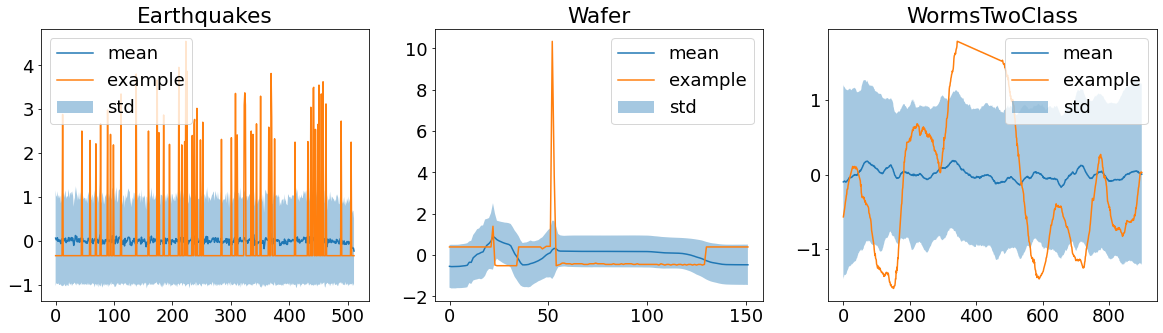
\includegraphics[width=0.9\textwidth, keepaspectratio=True]{figures/ds_visualization.png}
    \caption{Visualization of the three datasets. For each dataset, we plot the average time series, the standard deviation at each timestamp and an example sampled randomly from the dataset.}
    \label{fig:ds_visulization}
\end{figure}

% \begin{table}
%     \centering
%     \begin{tabular}{c|c|c|c}
%          Name & Size & Length & Percentage of positive class \\
%          WormsTwoClass & 1 & 10 & 50
%     \end{tabular}
%     \caption{Caption}
%     \label{tab:my_label}
% \end{table}

\begin{figure}
    \centering
    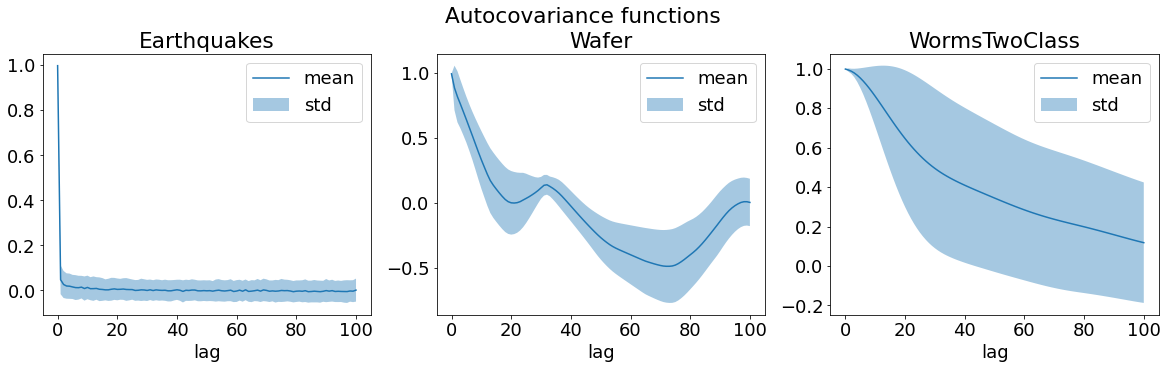
\includegraphics[width=0.9\textwidth, keepaspectratio=True]{figures/ds_acov.png}
    \caption{Average autocovariance functions for the three datasets.}
    \label{fig:ds_acov}
\end{figure}

\paragraph{The features} Finally, since feature extraction is not the task we are interested in here, we used TSFEL \cite{barandas_tsfel_2020}, a library specialized in feature extraction from time series. The number of features extracted per series depends on the time series, and in the case of our data it varies between 210 and 389.

\newpage
\section{Results}

\subsection{Impact of parameters $\sigma$ and $k$} 

\paragraph{Histograms of the Laplacian scores} First, we plot some histograms of the distributions of the Laplacian scores when sigma varies. To do so, we choose a dataset (here, the Wafer one), we fix the number of neighbors, for example to 25. Moreover, we focus on the ratio $\sigma / \overline{M}$, where $\overline{M}$ is the average of the values of $M$, which makes more sense than the raw value of sigma. The result can be seen in Figure \ref{fig:sigma_histograms}. We observe on this figure (and the similar ones for the other dataset, that are easy to generate with the notebook) that there are two quasi-stationary phases: one when $\sigma$ is really small, and one when $\sigma$ is really large. This is not surprising. With the notations of section \ref{sec:method}:

\begin{itemize}
    \item When $\sigma$ tends to zero, $S \rightarrow 0$, so $D \rightarrow 0$ and $L \rightarrow 0$. Given that we added a small $\varepsilon$ in the division for the computation of the Laplacian score, it is thus normal that the scores converge to zero. This corresponds to a situation when every point can only ``see" itself due to the Gaussian kernel.
    \item When $\sigma$ is really large, $S \rightarrow G$. This corresponds to a situation where all neighbors have the same importance due to the high radius of the Gaussian kernel. Thus, the Laplacian scores tends to their values with $S$ was perfectly equal to $G$.
\end{itemize}

\begin{figure}
    \centering
    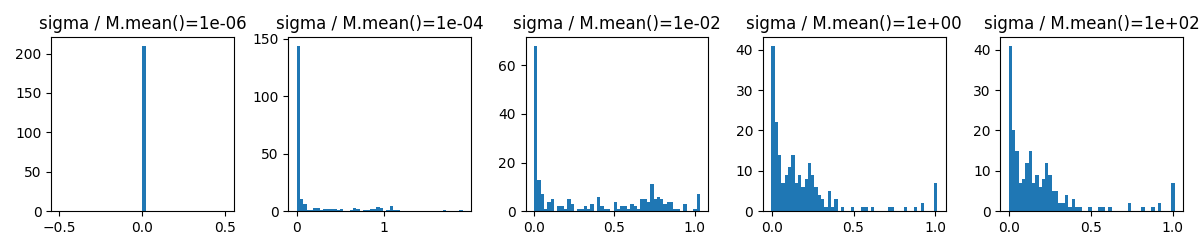
\includegraphics[width=\textwidth, keepaspectratio=True]{figures/laplacian_histograms.png}
    \caption{Histograms of the value of the Laplacian score for several values of $\sigma / \overline{M}$}
    \label{fig:sigma_histograms}
\end{figure}


\paragraph{Impact of $\sigma$ on the classification accuracy} These histograms allowed us to understand the general behavior of the score. However, to better understand the impact of $\sigma$, we directly measured its impact on the classification accuracy. To do so, we fixed the number of neighbors, and we made $\sigma$ vary between $10^{-7}$ and $10^{+3}$. We repeated this experiment with several values of the number of feature that were finally selected. The results are presented in figure \ref{fig:accuracy_vs_sigma}. We observe that:

\begin{itemize}
    \item For some datasets (namely, Wafer and Earthquakes), the accuracy is quite stable, no matter the value of $\sigma$ or the number of features selected. This is probably because the classification problem is either too simple or too hard with the features we have. For example with dataset Earthquakes, we observe a performance of $0.8 \simeq 368/461$, which is the proportion of label ``1" in the dataset. No matter the features that are selected, they are not informative enough, and the best that can be done by the SVC is to predict the same label for every sample. 
    \item In most cases, the best performance comes for low sigma values, around $10^{-4}$. In the case of 150 features selected, the maximum is reached around $10^{-2}$, however this maximum is only equal to the maximum with 30 features. 
\end{itemize}

Thus, for the stability of the method, it is safe to always take a quite small value for $\sigma/\overline{M}$, yet not too small to to avoid that every Laplace score is equal to $0$.

\begin{figure}
    \centering
    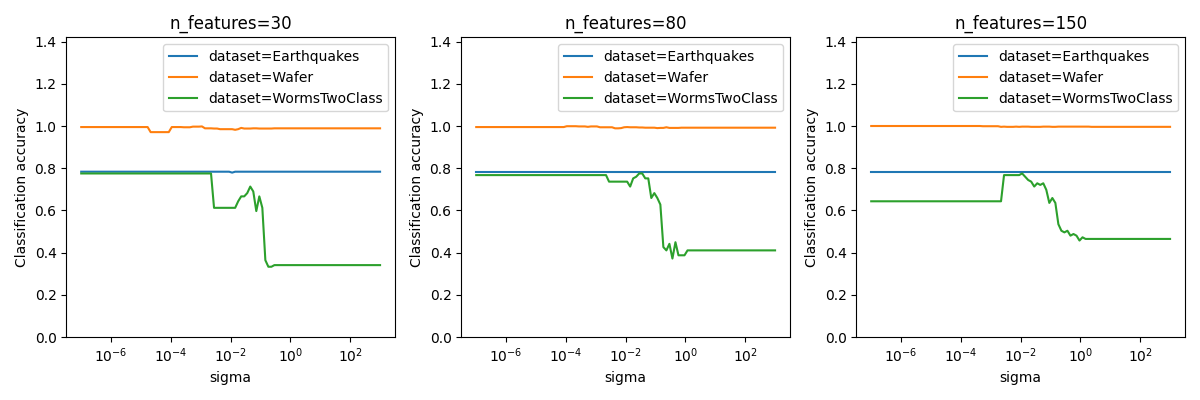
\includegraphics[width=0.80\textwidth]{figures/accuracy_vs_sigma.png}
    \caption{Evolution of the classification accuracy against the value of $\sigma / \overline{M}$.}
    \label{fig:accuracy_vs_sigma}
\end{figure}

\paragraph{Impact of the number of neighbors $k$ on the classification accuracy}

Then, we measured the impact of the number of neighbors on the performances. The result is presented in figure \ref{fig:accuracy_vs_n_features}. We observe that if we stick to small values of $\sigma / \overline{M}$, the number of neighbors does not really the classification accuracy. To conclude, a good heuristic for the choice of $\sigma$ and $k$ is to take $\sigma / \overline{M}$ small enough, around $10^{-4}$, and $k$ medium, of the order of ten.

\subsection{Comparison with other methods}

Finally, we compared this filter method with two other: a variance threshold (unsupervised), and the ANOVA score (supervised). The result is presented in Figure \ref{fig:accuracy_vs_n_features}. We observe that the method based on the Laplace score has similar performances to these two techniques, and is even better on certain ranges of values. However, for a limited number of features, the performance gap remains important, and constitutes a major disadvantage of the method. Finally, we observe that contrary to what we could have intuitively imagined, the performances are not improved, on the contrary, by using the DTW, and this even if DTW is generally considered more relevant for time series. 

\begin{figure}
    \centering
    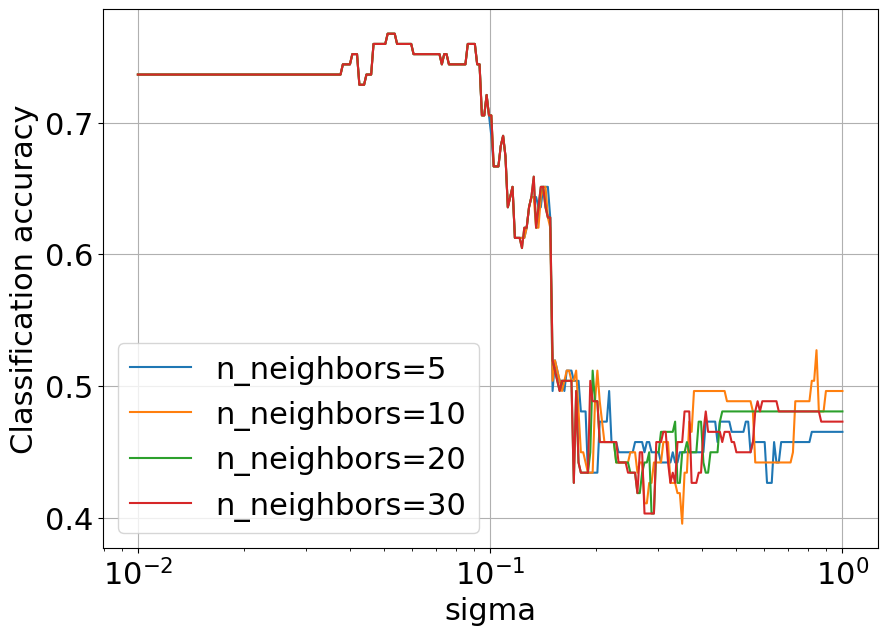
\includegraphics[width=0.35\textwidth]{figures/accuracy_vs_sigma_and_nnn.png}
    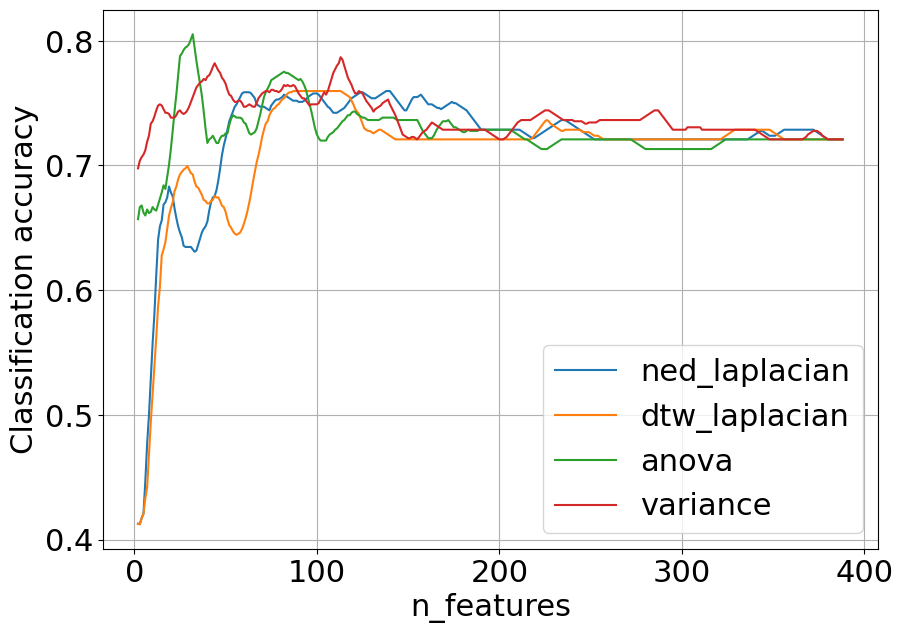
\includegraphics[width=0.35\textwidth]{figures/accuracy_vs_n_features.png}
    \caption{Left: Evolution of the classification accuracy against the value of sigma. Right: Evolution of the classification accuracy against the number of features.}
    \label{fig:accuracy_vs_n_features}
\end{figure}

\section{Conclusion}

Our experiments identified heuristics for choosing sigma and the number of neighbors in the absence of additional knowledge about the data. Moreover, our experiments have shown that this method leads to relatively good performances compared to other widely used methods such as the ANOVA score, although they remain slightly inferior.


%% The next two lines define the bibliography style to be used, and
%% the bibliography file.
\newpage
\bibliography{references}
\bibliographystyle{ACM-Reference-Format}

\end{document}
